\section{Durchführung}
\label{sec:Durchführung}

Der verwendete Versuchsaufbau ist in \autoref{fig:Versuchsaufbau} zu sehen.
Im wesentlichen besteht er aus einem $\beta$- oder $\gamma$-Strahler, einem
Geiger-Müller-Zählrohr und einer verstellbaren Aufnahme für Absorptionsplatten unterschiedlicher
Dicke. Außen ist der Versuch mit einer Pb-Abschirmung versehen, um die Strahlenbelastung möglichst
gering zu halten.
\begin{figure}[H]
    \centering
    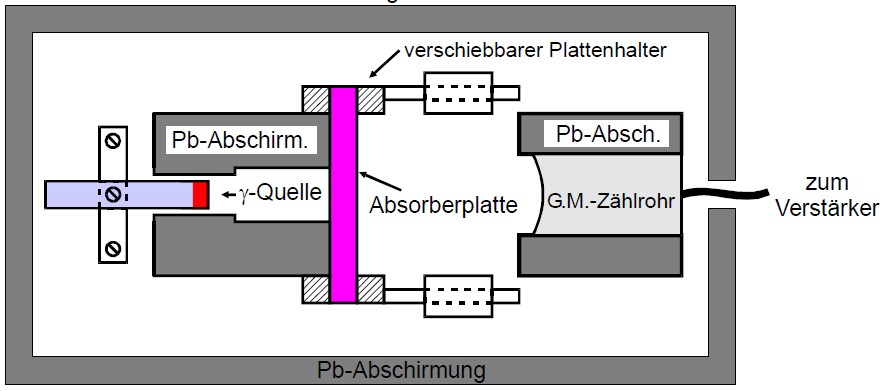
\includegraphics[height=5cm]{content/pics/versuch.jpg}
    \caption{Versuchsaufbau \cite{v704}.}
    \label{fig:Versuchsaufbau}
\end{figure}
Vor Beginn der eigentlichen Messung wird die Hintergrundstrahlung, auch Nullrate genannt, gemessen.
Dafür wird die Anzahl der ausgelösten Impulse im Geiger-Müller-Zählrohrs über einen Zeitraum von $\qty{900}{\second}$
bestimmt.

\subsection{\texorpdfstring{Absorptionsmessung von $\beta$-Strahlung}{Absorptionsmessung von Beta-Strahlung}}
\label{sec:seggs}
Nun wird der $\beta$-Strahler in den Versuchsaufbau platziert, für diesen Versuch wird Technezium-99 verwendet.
Bevor ein Absorber zwischen Strahler und Zählrohr hinzugefügt wird, soll noch eine Nullmessung ohne jegliche
Absorption durchgeführt werden.
Anschließend wird Aluminium als Absorber zwischen Strahler und Zählrohr platziert, dessen Dicke
je Messung schritttweise erhöht wird.
Als Messzeitintervall wird ein Wert zwischen $\qty{200}{\second}$ und $\qty{400}{\second}$ gewähnt, der 
mit steigender Dicke ausgehend von $\qty{200}{\second}$ langsam erhöht werden sollte.
Insgesamt werden 10 verschiedene Dicken gemessen.

\subsection{\texorpdfstring{Absorptionsmessung von $\gamma$-Strahlung}{Absorptionsmessung von Gamma-Strahlung}}
Auch hier wird wie in \autoref{sec:seggs} beschrieben zuerst eine Nullmessung durchgeführt.
Zur Erzeugung der $\gamma$-Strahlung wird ein Cäesium-137 Präperat verwendet.
Das Messzeitintervall wird wie in \autoref{sec:seggs} variert, jedoch soll der Wert hier zwischen
$\qty{100}{\second}$ und $\qty{200}{\second}$ liegen.
Als Absorber werden Blei und Zink verwendet, beide liegen in Form von unterschiedlich dicken Metallplatten vor.
Durch Kombination dieser Platten werden je Absorber 10 verschiedene Dicken erzeugt und die Zählraten gemessen.